\documentclass[12pt,letterpaper]{article}

\newenvironment{proof}{\noindent{\bf Proof:}}{\qed\bigskip}

\newtheorem{theorem}{Theorem}
\newtheorem{corollary}{Corollary}
\newtheorem{lemma}{Lemma} 
\newtheorem{claim}{Claim}
\newtheorem{fact}{Fact}
\newtheorem{definition}{Definition}
\newtheorem{assumption}{Assumption}
\newtheorem{observation}{Observation}
\newtheorem{example}{Example}
\newcommand{\qed}{\rule{7pt}{7pt}}

\newcommand{\assignment}[4]{
\thispagestyle{plain} 
\newpage
\setcounter{page}{1}
\noindent
\begin{center}
\framebox{ \vbox{ \hbox to 6.28in
{\bf CS446: Machine Learning \hfill #1}
\vspace{4mm}
\hbox to 6.28in
{\hspace{2.5in}\large\mbox{Problem Set #2}}
\vspace{4mm}
\hbox to 6.28in
{{\it Handed Out: #3 \hfill Due: #4}}
}}
\end{center}
}

\newcommand{\solution}[4]{
\thispagestyle{plain} 
\newpage
\setcounter{page}{1}
\noindent
\begin{center}
\framebox{ \vbox{ \hbox to 6.28in
{\bf CS446: Machine Learning \hfill #4}
\vspace{4mm}
\hbox to 6.28in
{\hspace{2.5in}\large\mbox{Problem Set #3}}
\vspace{4mm}
\hbox to 6.28in
{#1 \hfill {\it Handed In: #2}}
}}
\end{center}
\markright{#1}
}

\newenvironment{algorithm}
{\begin{center}
\begin{tabular}{|l|}
\hline
\begin{minipage}{1in}
\begin{tabbing}
\quad\=\qquad\=\qquad\=\qquad\=\qquad\=\qquad\=\qquad\=\kill}
{\end{tabbing}
\end{minipage} \\
\hline
\end{tabular}
\end{center}}

\def\Comment#1{\textsf{\textsl{$\langle\!\langle$#1\/$\rangle\!\rangle$}}}



\usepackage{graphicx,amssymb,amsmath, listings}
\lstset{language = Matlab}
\lstset{breaklines}
\usepackage{float}
\lstset{extendedchars=false}

\oddsidemargin 0in
\evensidemargin 0in
\textwidth 6.5in
\topmargin -0.5in
\textheight 9.0in
\begin{document}

\solution{Jifu Zhao}{\today}{3}{Fall 2015}
% Fill in the above, for example, as follows:
% \solution{Joe Smith}{\today}{1}{Fall 2012}

\pagestyle{myheadings}  % Leave this command alone

\begin{enumerate}
\item {\bf Answer to Experiment 1}\\

In this problem, there are two dataset for the problem. One with l = 10, m = 100, n = 500 and another with l = 10, m = 100, n = 1000. First, using the gen.m, I got two clean data with 50,000 examples for each group. Then, after randomly choosing 10\% as training set and another distinct 10\% as the test set. I successfully tuning the parameters for these five algorithms. The result is shown in Table 1.\\

\begin{table}[H]
\caption {Experiment 1 paremeters tuning result} \label{tab:title} 
  \begin{center}
    \begin{tabular}{|p{3.0cm}|p{2.2cm}|p{2.5cm}|p{2.5cm}|p{2.5cm}|}
      \hline
      Algorithm & Parameters & Dataset n=500 & Dataset n=1000\\\hline\hline
      Perceptron & None &  &  \\\hline
      Perceptron w/margin & $\eta$ & 0.005 & 0.03 \\\hline
      Winnow & $\alpha$& 1.1 &  1.1    \\\hline
      Winnow w/margin & $\alpha$, $\gamma$ & 1.1, 2.0 &  1.1, 0.04 \\\hline
      AdaGrad & $\eta$ & 0.25 &  0.25 \\\hline
    \end{tabular}
  \end{center}
\end{table}

  
{\bf Note:} when n = 1000, for the Winnow with margin algorithm, the accurate can be the same for the chosen training and test data set with $\gamma$ = 0.04 or $\gamma$ = 0.006. But there, we just choose $\gamma$ = 0.04.\\

Having got the best parameters, the next step is to using these parameters and run the five algorithms on the dataset with 50,000 examples.\\

{\bf First,} run the five algorithm with l = 10, m = 100, n = 500. The result is shown in Figure 1.\\

\begin{figure}[H] 
\begin{center}
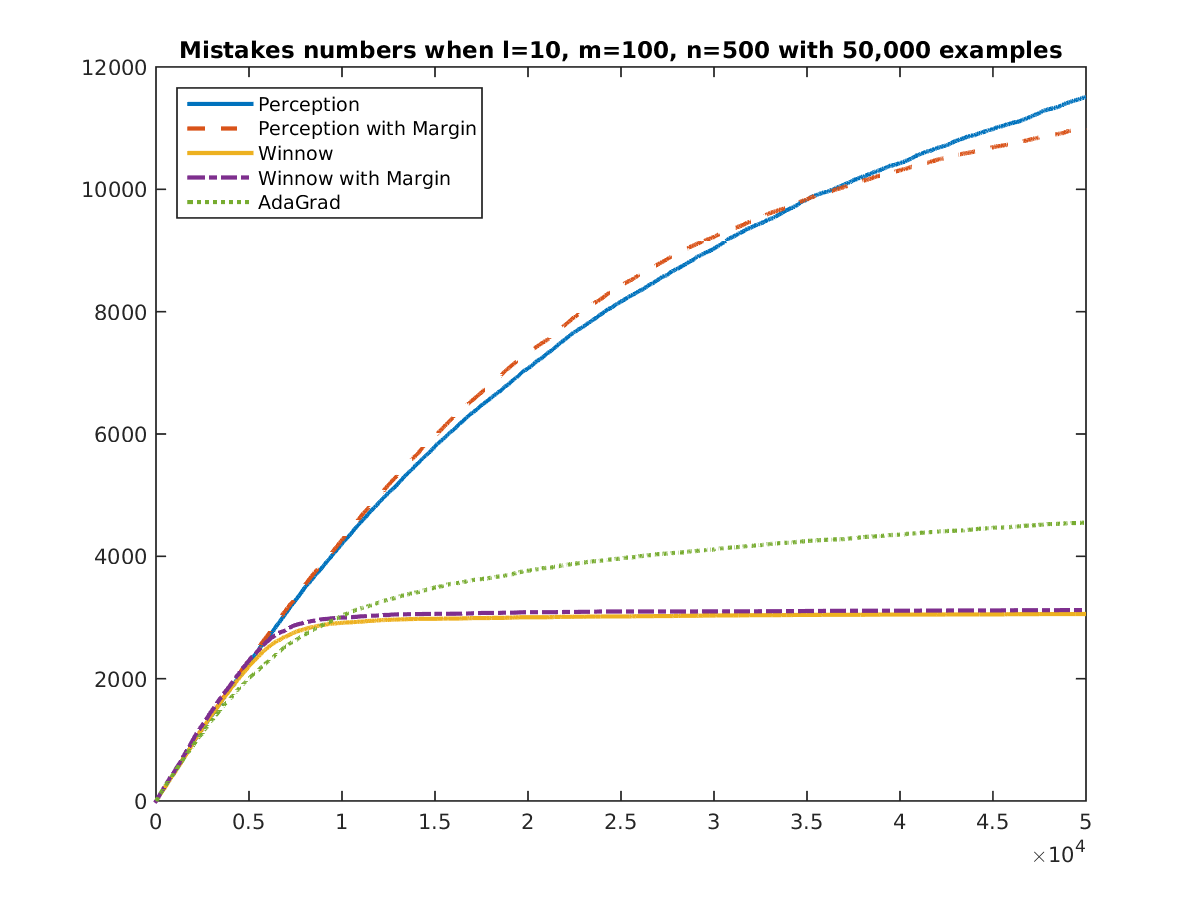
\includegraphics[width=7in]{Ex1mistake1.png}
\caption{l = 10, m = 100, n = 500, N = 50,000}
\end{center}
\end{figure}

In this figure, we use 50,000 examples. But for Perception and Perception with Margin algorithms, the convergence is not very clear. So, I changed the examples from 50,000 to 250,000, the result is shown in Figure 2.\\

\begin{figure}[H] 
\begin{center}
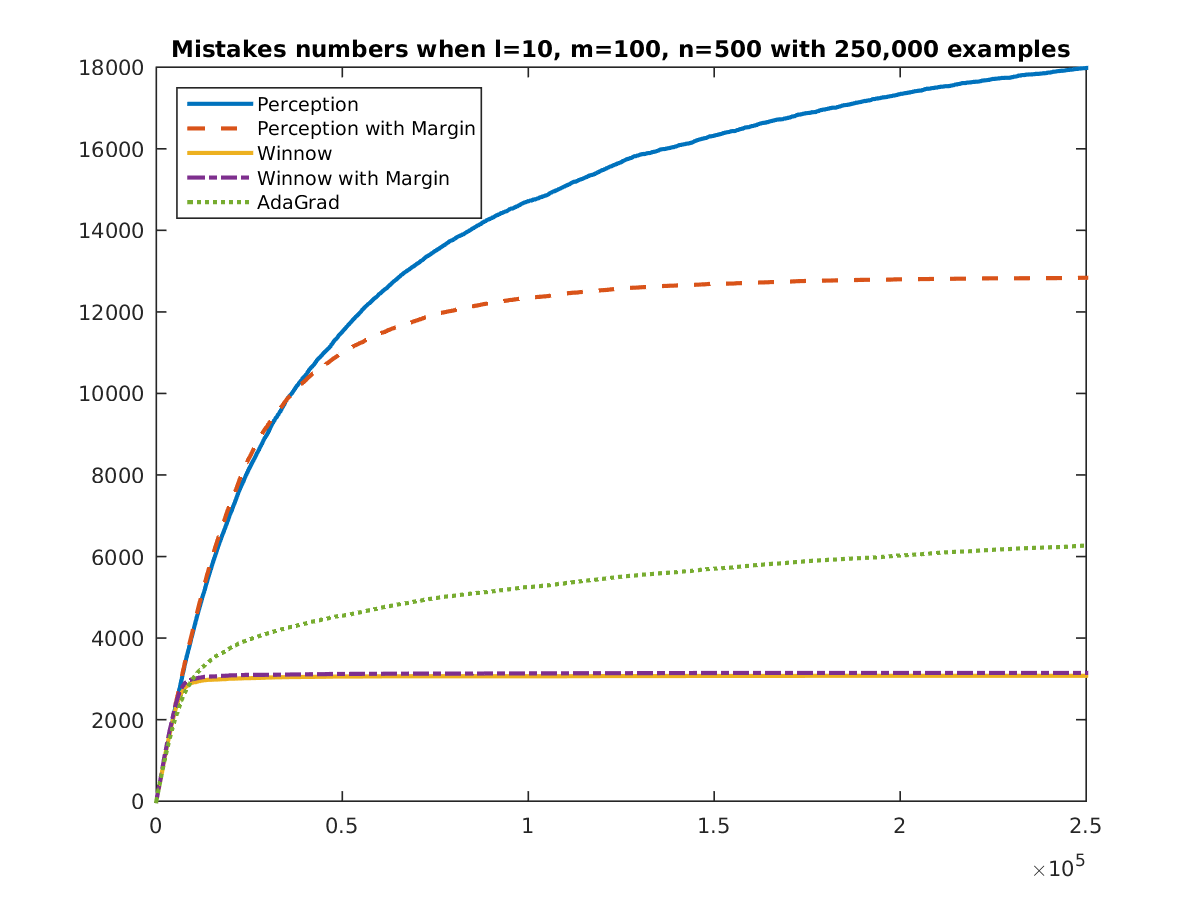
\includegraphics[width=7in]{Ex1mistake2.png}
\caption{l = 10, m = 100, n = 500, N = 250,000}
\end{center}
\end{figure}

In Figure 2, the result looks much better.\\

{\bf Next,} run the five algorithm with l = 10, m = 100, n = 1000. The result is shown in Figure 3.\\

\begin{figure}[H] 
\begin{center}
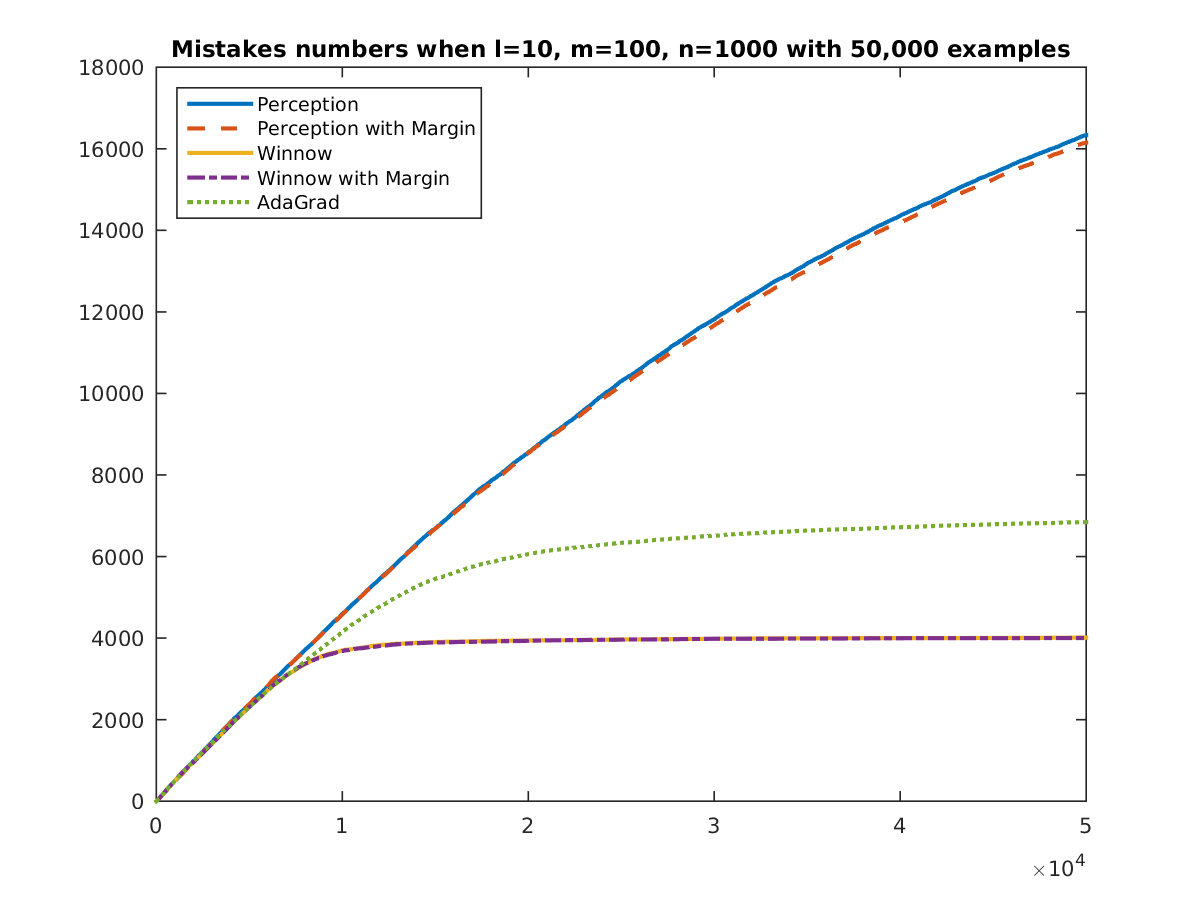
\includegraphics[width=7in]{Ex1mistake3.png}
\caption{l = 10, m = 100, n = 1000, N = 50,000}
\end{center}
\end{figure}

The same problem appears again, the convergence is not very clear for Perception and Perception with Margin algorithms. So, I changed the examples from 50,000 to 250,000, the result is shown in Figure 4.\\

\begin{figure}[H] 
\begin{center}
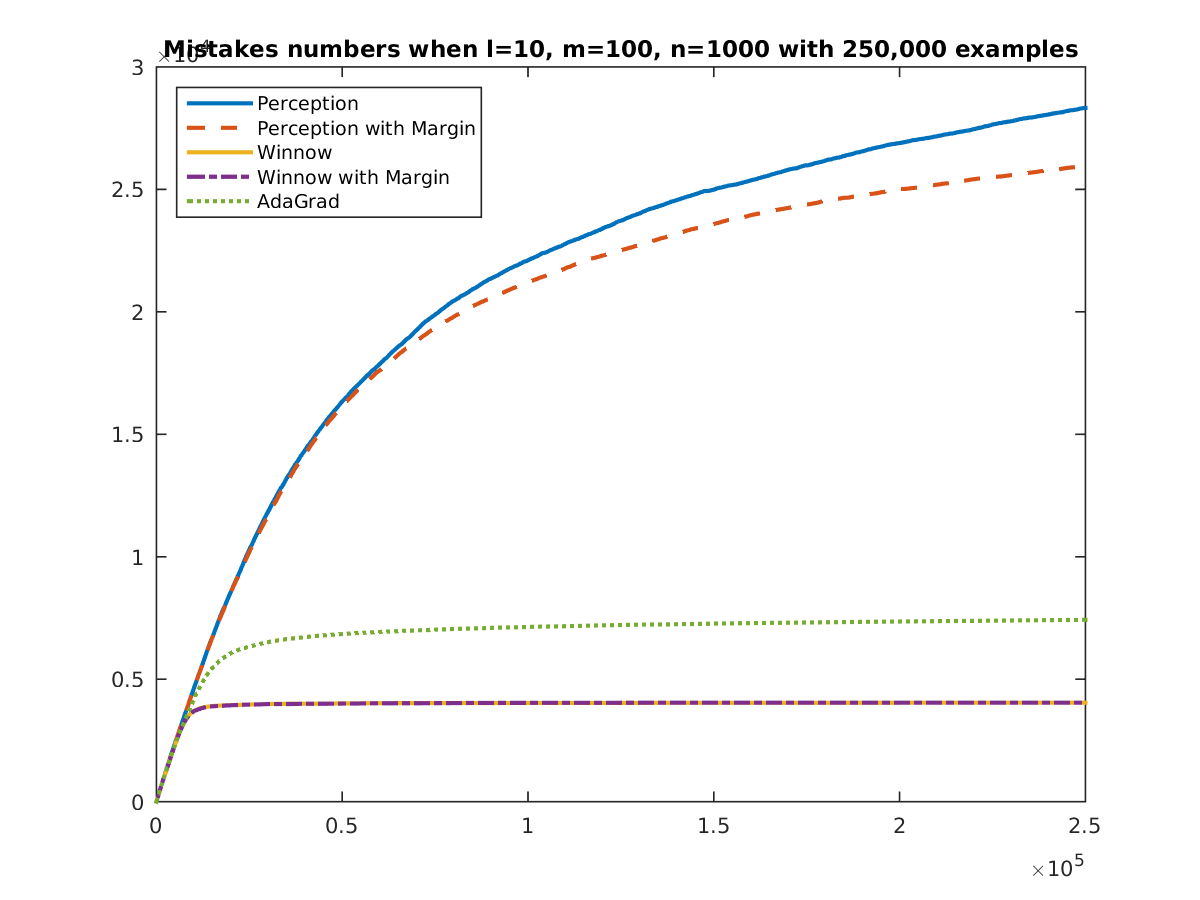
\includegraphics[width=7in]{Ex1mistake4.png}
\caption{l = 10, m = 100, n = 1000, N = 250,000}
\end{center}
\end{figure}

{\bf Discussion:\\}

Comparing the Figure 1, 2, 3 and 4, we can find that as the number of examples increases, the number of mistakes will all increase for five algorithms. They will finally converge. However, their change trend is different. For Winnow and Winnow with Margin algorithm, they converge very fast. And AdaGrad algorithm converge a little slower than Winnow and Winnow with Margin algorithms. And Perception and Perception with Margin algorithms converge very slow. Of course, Perception with Margin behaves a little better than Perception algorithm. It makes less mistakes. From the point of making mistakes, Winnow, Winnow with Margin and AdaGrad have much better performance than Perception and Perception with Margin.\\


\item {\bf Answer to Experiment 2}\\

For this question, we have five group of data with n equals 40, 80, 120, 160 and 200. Using the same procedure in Experiment 1, I have successfully tuning the parameters. The result are shown in Table 2.\\

\begin{table}[H]
\caption {Experiment 2 paremeters tuning result} \label{tab:title} 
  \begin{center}
    \begin{tabular}{|p{3.0cm}|p{2.2cm}|p{1cm}|p{1cm}|p{1cm}|p{1cm}|p{1cm}|}
      \hline
      Algorithm & Parameters & n=40 & n=80 & n=120 & n=160 & n=200\\\hline\hline
      Perceptron & None &  &  & & &\\\hline
      Perceptron w/margin & $\eta$ & 0.25 & 0.25 & 0.25 & 0.03 & 0.03 \\\hline
      Winnow & $\alpha$& 1.1 & 1.1 & 1.1 & 1.1 & 1.1 \\\hline
      Winnow w/margin & $\alpha$, $\gamma$ & 1.1, 2.0 &  1.1, 2.0 & 1.1, 0.001 & 1.1, 0.001 & 1.1, 2.0 \\\hline
      AdaGrad & $\eta$ & 1.5 & 1.5 & 1.5 & 1.5 & 1.5 \\\hline
    \end{tabular}
  \end{center}
\end{table}

{\bf Note:} For each algorithm, there will be several parameters that can result the highest accuracy with same value. To simplify the following process, I just select one of them.\\

Having got the best parameters, the next step is to running the algorithms on the dataset with 50,000 examples. Through set the right case number R to be 1,000, I recorded the number of mistakes W for each algorithm. The result is shown in Figure 5.\\

\begin{figure}[H] 
\begin{center}
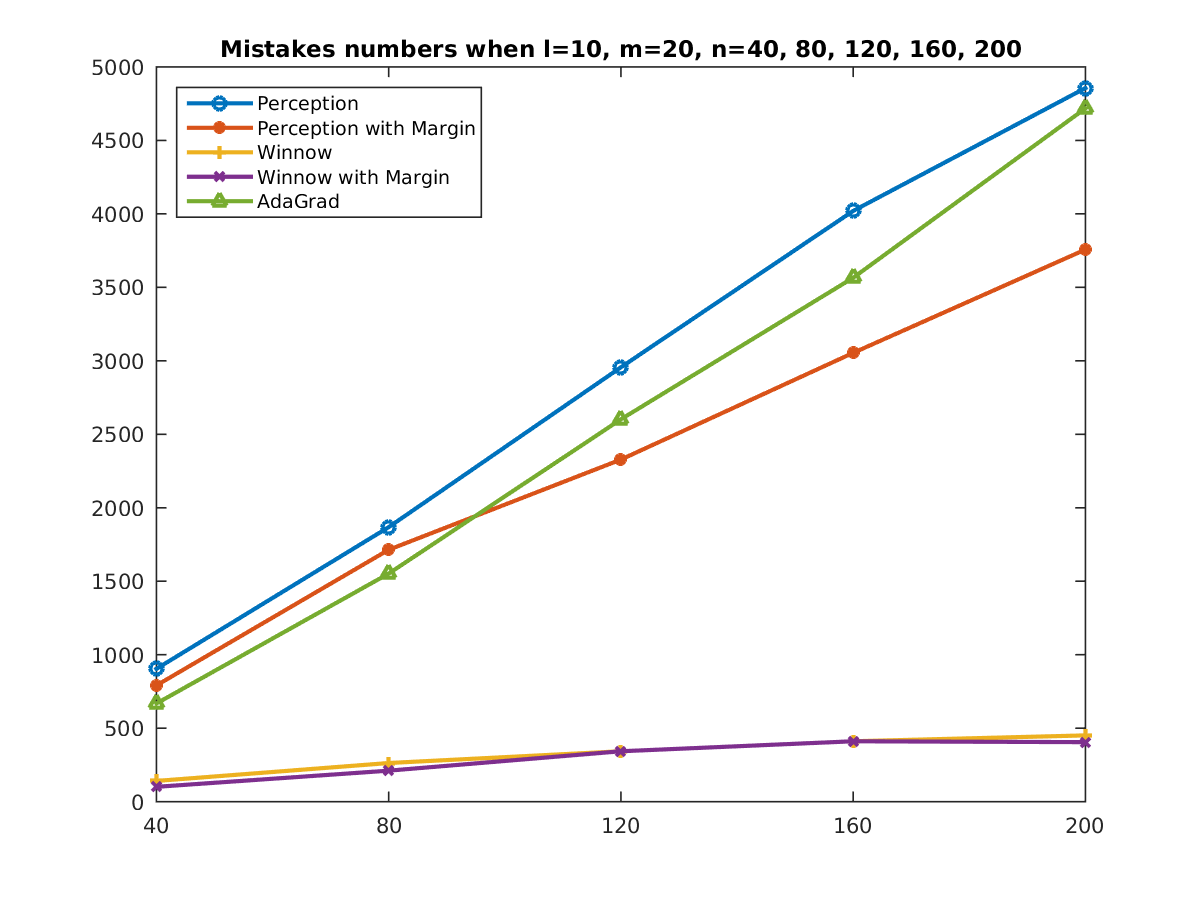
\includegraphics[width=7in]{Ex2mistake1.png}
\caption{Experiment 2 result}
\end{center}
\end{figure}

{\bf Discussion:\\}
In Figure 5, the performance of Winnow and Winnow with Margin algorithms are consistent with our expectation. They make least mistakes. This is consistent with Figure 1, 2, 3 and 4. Also, the performance of Perception and Perception with Margin algorithms look just fun. Their number of mistakes is much higher than Winnow and Winnow with Margin algorithms. However, for AdaGrad algorithm, its performance is not consistent with expectation. As expected, its mistakes should be between Winnow and Perception. However, in Figure 5, its mistakes numbers is much higher than expected. The possible explanation for this phenomena is that: during the experiment, there is several combinations of parameters that result in the same accuracy. However, I just randomly select one of them to run the algorithm over the whole dataset. It is possible that the parameters that I choose is actually not the best one for the whole dataset. Another possible explanation can be that: during the process of randomly select the 10\% data as training as test data, the data I choose, by accidentally, is not a good represent for the whole data. (But the possibility for this is really low.) The possible solution for this is to change the training and test data, and also, try different combination of parameters.\\

\item {\bf Answer to Experiment 3}\\

In this experiment, I first successfully generate two dataset, one have 50,000 examples with noise and another one have 10,000 examples without noise. Using the same procedure, I successfully tuning the parameters. The result is shown in Table 3.\\

\begin{table}[H]
\caption {Experiment 3 paremeters tuning result} \label{tab:title} 
\begin{center}
  \begin{tabular}{|p{3.0cm}|l|p{2.2cm}|l|p{2.2cm}|l|p{2.2cm}|}
\hline
 Algorithm &  \multicolumn{2}{c|}{m=100} & \multicolumn{2}{c|}{m=500} & \multicolumn{2}{c|}{m=1000}\\\hline\hline
 & acc. & params. & acc. & params. & acc. & params.\\\hline
 Perceptron          & 0.9600 & None &  0.7524 & None & 0.7347 & None\\\hline
 Perceptron w/margin & 0.9956 & $\eta=0.005$ & 0.8091 &$\eta=0.005$ & 0.8125 & $\eta=0.03$ \\\hline
 Winnow              & 0.9599 & $\alpha=1.1$ & 0.8522 & $\alpha=1.1$ & 0.7453 & $\alpha=1.1$ \\\hline
 Winnow w/margin     & 0.9611 & $\eta=1.1, \gamma=0.006$ & 0.8041 & $\eta=1.1, \gamma=0.04$ & 0.7479 & $\eta=1.1, \gamma=0.001$ \\\hline
 AdaGrad             & 0.9996 & $\eta=0.25$ & 0.8931 & $\eta=1.5$ & 0.8173 & $\eta=1.5$ \\\hline
\end{tabular}
\end{center}
\end{table}

{\bf Discussion:\\}
Choosing the best parameters, I evaluate the algorithms on the test data with 10,000 examples, the accuracy is also shown in Table 3. As you can see in Table 3, when m = 100, all algorithms have good performance, especially the AdaGrad algorithm. Its accuracy can be 99.96\%. However, when m increases, the performance for the five algorithms decrease very clearly. Especially the Perception algorithm, its accuracy decreases most. Comparing these five algorithms, we can find that AdaGrad algorithms have the best result and Perception algorithm have the worst result. This is different from the result of experiment 2, in which Winnow and Winnow with Margin have the best performance. So, with noise data, the performance of different algorithms will also change.\\

\item {\bf Answer to Experiment 4}\\

For the {\bf Basic Perceptron} algorithm, there is only one parameter--learning rate $\eta$. However, only change $\eta$ will not significantly change the accuracy. So, compared with the {\bf Perceptron with margin} algorithm,  I find that we can also set a margin $\gamma$ for this question. However, when I change the gamma, the result is not very ideal. So, I realized that only set one $\gamma$ is not enough. Since, $y$ belongs to $\{1, -1\}$, I realized that maybe we can set two $\gamma$ parameters $\gamma_+$ and $\gamma_-$. In this way, I got some results that looks good enough. \\

For {\bf learning rate $\eta$}, I set that
\begin{center}
$\eta = \{1.5, 0.25, 0.03, 0.005, 0.001 \}$\\
$\gamma_+ = \{1.0, 0.5, 0.1, 0.05, 0.01, 0.005, 0.001 \}$\\
$\gamma_- = \{1.0, 0.5, 0.1, 0.05, 0.01, 0.005, 0.001 \}$.
\end{center}
 Through combine these three parameters, I did 245 experiments and find the most suitable parameters for this question.
 
\begin{table}[H]
\caption {Experiment 4 paremeters tuning result} \label{tab:title} 
    \begin{center}
  \begin{tabular}{|p{3.8cm}|l|p{2.2cm}|l|p{2.2cm}|l|p{2.2cm}|}
\hline
 Algorithm &  \multicolumn{2}{c|}{m=100} & \multicolumn{2}{c|}{m=500} & \multicolumn{2}{c|}{m=1000}\\\hline\hline
 & acc. & params. & acc. & params. & acc. & params.\\\hline
 Perceptron          & 0.8883 & $\eta=1, \gamma=0$ &  0.8239 & $\eta=1, \gamma=0$ & 0.9753 & $\eta=1, \gamma=0$\\\hline
 Modified Perceptron & 0.9000 & $\eta=0.001$ $\gamma_+=0.005$ $\gamma_-=1.000$ & 0.9000 & $\eta=0.001$ $\gamma_+=1.000$ $\gamma_-=1.000$ & 0.9912 & $\eta=0.001$ $\gamma_+=0.005$ $\gamma_-=0.005$ \\\hline
\end{tabular}
\end{center}
\end{table}

As you can see from Table 4, after changing the parameters of $\eta$, $\gamma_+$ and $\gamma_-$, the accuracy change clearly.\\

\end{enumerate}

\end{document}

